\chapter{New solutions for task migration\label{chap:data_struct_dev}}

In this chapter we will explain several solutions designed to improve the
scalability of the task migration algorithms. Our analysis will be related 
to new data structures and new concurrency management solutions.

\section{Skip list\label{Skiplist}}

Common abstract data types like ordered lists are usually implemented through
a binary tree or through a sort of balanced tree. The former is simple
to develop and mantains good performance except when some particular sequences of
operations are performed on it. An example of such a sequence is the inserting 
of elements in order: in such a scenario the tree becomes a degenerated data structure
that has very poor performance. The latter has a similar behaviour but, with
a more complicated algorithm, it tries to mantain certain balance conditions
to ensure good performance. Obviously, we have to pay this benefit
with a certain overhead that affects all operations performed on the self-balanced
tree
.
It is possible to observe that the number of ``bad'' sequences are low: so, if it
were possible to randomly permute the list of items to be inserted, trees would work
well with high probability for any input sequence. Unfortunately, in most cases,
queries are answered ``online'', so randomly permuting the input is impractical.

\emph{Skip lists} are a probabilistic alternative to balanced trees: they are
balanced by consulting a random number generator. Although skiplists have bad
worst-case performance, no input sequence consistently produces the worst-case
performance, as observed in~\cite{Pugh}.

\subsection{Skip List structure and asymptotic complexity}
A skip list is capable to store a sorted list of items using a hierarchy of linked
lists that connect increasingly (bottom-up) sparse subsequences of the items. An
example of its structure is visible in Figure~\vref{fig:skiplist}.

\begin{figure}[htbp]
    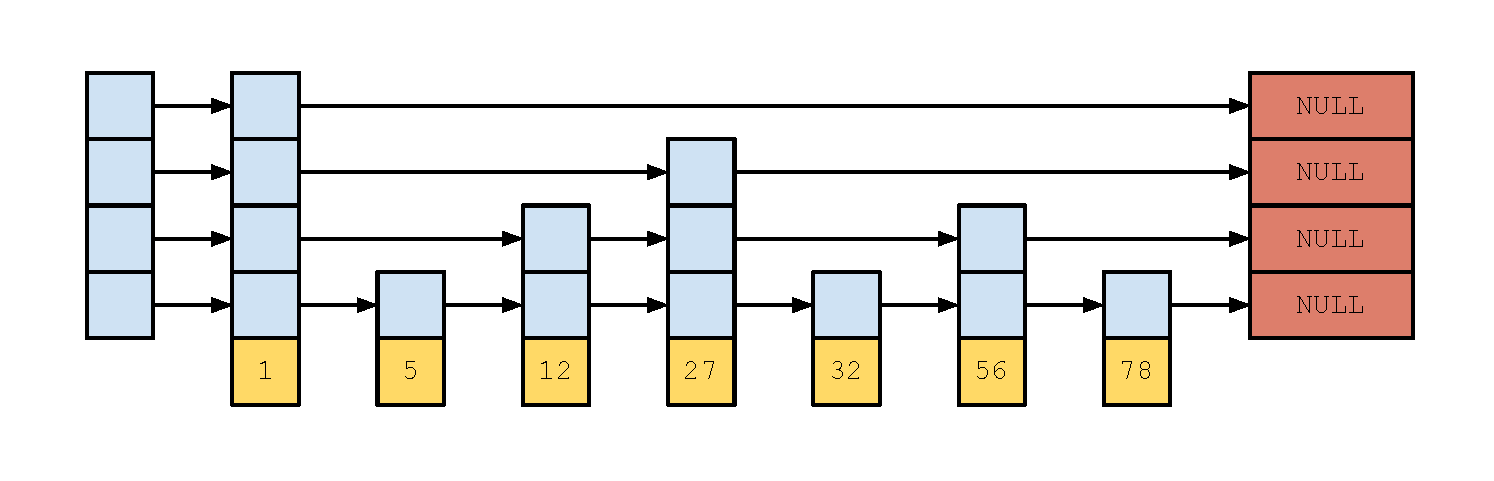
\includegraphics[width=\columnwidth]{images/Skiplist}
    \caption{An example skip list.}
    \label{fig:skiplist}
\end{figure}

Each link of the sparser lists skips over many items of the full list in one step, hence
the structure's name. These forward links may be added in a randomized way with some
kind of probability distribution, typically the geometric one.
Skip lists present the following operations complexity:

\begin{itemize}
\item Insert $\mathcal{O}(\log{n})$
\item Search $\mathcal{O}(\log{n})$
\item Delete $\mathcal{O}(\log{n})$
\end{itemize}

\noindent where \textit{n} is the number of items stored in the list.
A skip list is built in layers.
The bottom layer is an ordinary ordered linked list. 
Each higher layer contains extra pointers that permit to skip over 
intermediate nodes: an element in layer \textit{i} appears in layer
\textit{i+1} with some fixed probability \textit{p} (commonly used values
are $\frac{1}{2}$ and $\frac{1}{4}$). On average, each element appears in
$\frac{1}{(1-p)}$, and the tallest element (usually a special head element 
at the front of the skip list) in $\log_\frac{1}{p}{n}$ lists.

A search for a target element begins at the head element in the top list,
and proceeds horizontally until the current element is smaller than the
target. If the current element is equal to the target, it has been found.
Otherwise, if the current element is greater than the target, or the search
reaches the end of the linked list, the procedure is repeated after moving 
down vertically to the next lower list. The expected number of steps in each
linked list is at most $\frac{1}{p}$.

Therefore, the total \emph{expected} cost of a search is $\log_\frac{1}{p}{n}$,
that is, as we stated above, logarithmic. Skip lists also offer the possibility
to trade search costs against storage costs by choosing different values of
\textit{p}.

\subsection{\texttt{cpudl} skip list implementation\label{sec:cpudl_skiplist}}

In this section we will present an implementation of a skip list tailored to
be used in \texttt{SCHED\_DEADLINE} migration mechanism.

The data structure has to hold the deadline value of the tasks currently 
executing on the CPUs (to speed-up \emph{push} algorithm decisions) and the 
deadline value of the next tasks currently enqueued on the CPUs' runqueue
(to speed-up \emph{pull} algorithm decisions).

We have already seen in Section~\ref{sec:max_heap_cpudl} the API used to cope 
with a certain \texttt{cpudl} implementation. Since we are only modifying
\texttt{cpudl} itself while leaving (for now) the same \emph{push/pull}
mechanism, we decided to mantain the same API.

Now, we can make two insightful observations:

\begin{itemize}
\item regarding the \emph{find} operation, we can see that the callers are always
interested in picking up the first element of the data structures, that is, the
index of the best CPU to where to push or pull a task;
\item regarding the \emph{set} operation, we can see that the callers always indicate
the cpu index whose deadline related value has to be updated.
\end{itemize}

So, we chose the following design to improve the accesses to the data structure:

\begin{itemize}
\item all the lists that compose the data structure are doubly-linked. So, we can
traverse the skip list both forward and backward, starting from any item;
\item we allocate a set of skip list nodes, one for each CPU in the system, and
we definitively pin each node to a specific CPU. Doing so, we don't have to allocate
or free memory after kernel start-up;
\item all the skip list items are referenced by an array of pointers, so we can 
address an item simply knowing the index of the associated CPU;
\item when a CPU has no deadline task in its runqueue, that is, when the scheduler
running on that CPU calls \texttt{cpudl\_set} with \texttt{is\_valid} sets to zero,
we write a specific ``invalid'' value in the corresponding skip list node.
Consequently, we detach the node from the skip list.
This node will be ready for later use and it will be addressable through the array;
\item when a CPU has a deadline task in its runqueue, we can recover the associated
node through the array, store the new deadline value, and then insert it in
the skip list;
\item finally, when a scheduler instance running on a CPU needs to know which
CPU is the best for task migration, we only have to read the head element of
the skip list.
\end{itemize}

To guarantee the synchronization between the different scheduler instances that
issues operations on \texttt{cpudl} data structure, we used a simple 
\texttt{spinlock}. We have to point out that the lock must be acquired only for
the \emph{set} operation: the \emph{find} operation is always performed lock-free through
these simple steps:

\begin{itemize}
\item we copy the pointer to the skip list head node in a local variable;
\item we check if this pointer is \texttt{NULL}: if so, no runqueue holds
a deadline task;
\item otherwise we read the CPU index and we return it to the caller.
\end{itemize}

This design leads to the following asymptotic complexities:

\begin{itemize}
\item find $\mathcal{O}(1)$
\item set $\mathcal{O}(\log(n))$
\end{itemize}

\noindent where \texttt{n} is equal to the number of CPUs in the system.
The code for this \texttt{cpudl} implementation is reported in
Appendix~\ref{sec:cpudl_skiplist_code}.

\section{Lock-free skip list\label{sec:lock_free_skiplist}}

An implementation of a lock-free skip list is described in~\cite{Pugh1990}.
To realize such a skip list, the author starts from an insightful observation:
``the distribution of levels within a skip list effects only the performance
of operations, not their correctness''. So, to delete an element we simply
reduce the level of that element one step at a time, until the level is equal to one.
Then, we delete it from the level one linked list, which deletes the
element. If we think of a level zero element as an element that has no pointers
and is not in the list, we can think of the process of deletion as reducing
the level of an element down to zero. The lock-free insertions works similarly:
we first insert the element in the level one linked list, then build up the level
of the element as appropriate.

Unfortunately, this approach can not be easily extended to a doubly-linked skip list,
as needed in \texttt{SCHED\_DEADLINE} to rapidly access to an item associated
with a certain CPU. So, we decided to give up with lock-free skip list to
focus on another concurrency management solutions.

\section{Bitmap flat combining\label{sec:bitmap_flat_combining}}

Flat Combining framework has already been briefly described in 
Section~\ref{sec:flat_combining}.
Here we are going to present some improvements that aim at making the framework
suitable for \texttt{SCHED\_DEADLINE} integration.

\subsection{Flat combining implementation details\label{sec:flat_combining_details}}

Recall from the previous discussion that flat combining, as its name suggests,
combines multiple operations together to complete them with a single pass 
on the underlying data structure.
To accomplish this task, the framework relies on a list of publication records,
through which the threads can request operations on the data structure.

Also, the published records list is a shared data structure that needs
to be protected from concurrent accesses. In the original framework design,
the authors suggest to use a linked list, with some devices to reduce contention:

\begin{itemize}
\item the list can not be left empty: at least one publication record must 
always be enqueued in it. This is useful to reduce contention between the combiner
and the others thread: the former always scans the list from the head, the latter
adds publication records to the tail;
\item the publication records have a field that indicates if the requested operation 
is completed. So, even if the combiner must leave a record in the list, it knows 
that there are no more operations to complete;
\item to avoid critical races when multiple threads add records to the list, we
use a \emph{CAS} operation on the tail of the list: this prevent us to
use a lock that may quickly become a performance bottleneck as the number of
threads increases;
\item finally, to balance the work between threads, the authors of the original
paper~\cite{Hendler2010} suggest to add
an \emph{aging} mechanism. In this way, every publication record has an age
field that is initialized when the record is published. The combiner thread,
while scanning the list, discards the old records. The publisher thread has to
periodically check if the requested operation is completed, otherwise he has
to publish again the record. 
\end{itemize}

The publication records list is crucial for flat combining performance. Suppose
that we have to perform a set of \emph{insert} operations on the data structure:
to ``combine'' the operations and insert multiple values at a time, the combiner
thread needs to sort the publication records list first. In this way, it is
possible to insert all the values in the structure in only one pass, one value
after the other.

\subsection{\texttt{cpudl} bitmap flat combining implementation\label{sec:cpudl_bm_fc}}

To obtain a suitable implementation of the flat combining framework, we bring some
improvements to the publication records list. Obviously, it was not possible to
use the framework ``as is'' in \texttt{SCHED\_DEADLINE}: the publication records
list would have soon arised scalability issues, both for the contention while adding
new records and for the sorting of all requests prior to execute the ``combined'' 
operations. Moreover, it is not possible to use an asynchronous programming model
inside push and pull operations: whenever a scheduler instance running on a CPU
has to migrate a task, it needs to know immediately which runqueue to choose.

It was decided to implement the publication records list as a hierarchical bitmap.

The top layer is a 64-bits bitmap: each bit is associated to a CPU in the system. 
Whenever a CPU has at least one publication record active, the corresponding
bit in the 64-bits bitmap is set.

The bottom layer is made of a set of 32-bits bitmap, one for each CPU. Every 32-bits
bitmaps keep tracks of the records published by a CPU (more precisely, by a scheduler
instance running on a CPU). So, in this implementation, every CPU can publish at
most 32 operations at a time.

As in the \texttt{cpudl} skip list implementation,
all the publication records are pre-allocated at kernel start-up and freed only 
at system shutdown: no overhead due to memory management will slow down the migration
mechanism.

The main reason to use bitmaps to arrange the publication records is the speed of the
functions that operate on them. In fact, almost every modern architecture provides, in its 
Instruction Set, a mean to know which is the first or the last bit set in such a bitmap.
Since these operations are hardware-implemented, they are usually very fast. In the
\emph{C POSIX Library} we found the function:

\begin{center}
\texttt{int ffs(int i);}
\end{center}

\noindent that operates on an \texttt{int} variable. The \emph{GNU C Library} adds the following
two functions that operates on arguments of possibly different size:

\begin{center}
\texttt{int ffsl(long int i);}\\
\texttt{int ffsll(long long int i);}
\end{center}

These functions all do the same thing: starting from the least significant bit in the
argument, they search for a set bit and, if found, the position is returned, otherwise
they return zero.

Also the Linux kernel provides two functions that do the same thing, except that they
return the most significant set bit in the argument. For our purpose, this different
behaviour is peddling. The functions are:

\begin{center}
\texttt{int fls(int x);}\\
\texttt{int fls64(u64 x);}
\end{center}

As discussed in Section~\ref{sec:mem_barriers}, to ensure that the sequence of write 
operations on the top level and the bottom level bitmaps made by a CPU will be 
perceived by all other CPUs in the same order, a write memory barrier has to be issued.
Similarly, the combiner CPU, while traversing the list, has to issue a paired read 
memory barrier.

Regarding the lock that protects the underlying data structure, it was decided to 
implement it through an \texttt{atomic\_t} variable. 
The lock is acquired with a simple \emph{CAS} operation, therefore with an 
\texttt{atomic\_cmpxchg()}. Note that, as stated in Section~\ref{sec:atomic_ops}, 
this operation issues an implicit memory barrier, so there is no way that the 
critical section instructions will be reordered and positioned prior to the 
locking instruction. For the same reason, when we release the lock, we use an 
\texttt{atomic\_set} operation and, after that, we issue a write
memory barrier. This design allows us not to deal with irqs mask saving and restore,
so it is a little faster than the \texttt{spinlock} solution.

As stated in the previous section, the flat combining framework introduces an
asynchronous programming model. This model is unacceptable for both the \emph{find}
and the \emph{set} operation.
Regarding the former operation, we introduce a cache
to always keep an updated value of the best CPU index where to migrate a task. Every
time a CPU do a \emph{set} operation, it checks the cached value and compare its
deadline to decide if the cache has to be updated. If so, a \emph{CAS} operation is
immediately performed and, after that, the record is published.

Regarding the latter operation, it was decided to restrict the maximum number of records
that a CPU can publish without waiting for the work to be done. In the actual 
implementation, this parameter can be varied changing the value of the macro 
\texttt{PUB\_RECORD\_PER\_CPU}, ranging from 1 to 32.

Finally, regarding the mechanism of ``combining'' the \emph{set} operations, here we can not
apply such a strategy. If we compare the mean number of such operations with the
number of elements in the underlying data structure (that is, the number of
CPUs in the system) we can easily understand that it is not worth to sort the 
requests to apply that in a single pass. Anyhow, using a combiner thread that
does all the work, we can benefit from keeping the cache hot in the combiner CPU, 
thus speeding up all the operations.

The code for this \texttt{cpudl} implementation is reported in
Appendix~\ref{sec:cpudl_bm_fc_code}.

\section{Fastcache\label{sec:Fastcache}}

Starting from the flat combining \texttt{cpudl} implementation discussed above, we 
can lead some important considerations.

Most of the \emph{find} operations are answered through the cache. In fact, we
use the underlying data structure only to ``reconstruct'' the cache when it is
invalidated. With such a design we can reach very high performance in the \emph{find}
operation. Unfortunately, the \emph{set} operation doesn't experiment a
similar boost: as we will see in Section~\ref{sec:bm_fc_perf}, the CPU cycles needed to complete
a \emph{set} is in the same order than the skip list solution.

This drawback can be addressed using a different design that aim to use as much as
possible the cache, to avoid complex algorithms that are not well suited to manage
a low number of items.

A common design pattern used in parallel programming to develop scalable algorithms
consists of separating the code path depending on how the concurrent requests on 
the data structure are interleaved. Typically we have a \emph{fast path}, where no lock
is taken, and a \emph{slow path}, where we must take some kind of lock to ensure the
correctness of the implementation. If we can ensure that the fast path will be
taken most of the time, thus leads to a very fast solution.

Regarding the \emph{set} operation on the \texttt{cpudl} data structure, recall 
from the discussion above that we already implicitly defined what we consider the
fast path: when a CPU finds the cache in a valid state, it can
compare the cached valued with its deadline value to update it, if needed. Since
the update is performed through atomic operations, no lock will be taken. If the
cache must not be updated, we are still in a path where no lock is needed.

A slow path must be followed when a \emph{set} operation takes place and the 
cached CPU is just the same that calls the function. In this case, the value
of the deadline related to that CPU must be updated, and we can not know if
another CPU holds a better deadline value. So, we need to rely on a data structure
where the deadline of all CPUs are stored to find which is the best one at the
time. Since multiple CPUs can call the \emph{set} operation concurrently, we have
to ensure that only one CPU will be authorized to manipulate the cache, in other
words, we need to protect the slow path with a lock.

For our purpose, we choose to implement the underlying structure with a simple
array, to be searched with a sequential search. This choice may seem self-defeating
but, as the experiments in Section~\ref{sec:fastcache_perf} show, it is not. Such an array allows
a very fast update of the deadline value associated to each CPU in the system: an
\texttt{atomic\_set} plus a write memory barrier is enough. This means that the
\emph{fast path} is indeed very fast. Obviously, as the number of underlying
CPUs increases, the sequential search will be increasingly slower and so will
be the \emph{slow path}. However,
when the number of CPUs increases it is more likely that, between two subsequent
\emph{set} operations coming from the same CPU (the second of which would invalidate the cache), 
there will be another \emph{set} operation from a different CPU that instead updates the 
cache. This update will change the CPU index cached value, preventing the subsequent
\emph{set} operation from invalidating the cache. 
In this manner the slow path will be taken in very few cases.

To guarantee the consistency of the \emph{cpudl} data structure, we have
to ensure that:

\begin{itemize}
\item as soon as a CPU enters the \texttt{cpudl\_set} function, it has to
update its deadline value stored in the array with an \texttt{atomic\_set};
\item when more than one CPU concurrently executes the \texttt{cpudl\_set}
while the cache is invalidated, we first try to acquire the lock to refill
it, but, if the lock is taken, we simply retry until the cache is valid. This
way, we have a chance to ``fast-update'' the cache with our new deadline value
through a simple \emph{CAS}.
\end{itemize}

Finally, another improvement can be made to speed up the \emph{slow path}. Suppose that
the number of per-CPU tasks is low: this condition leads to a higher number
of runqueues with only one deadline tasks enqueued in it. So, we would have an
increasing rate of \emph{set} operations with the \texttt{is\_valid} flag set to zero, 
thus leading to a higher rate of cache invalidations. So, to obtain good performance even
in such a situation, we used the CPU bitmask also for the pull operation: while scanning
the deadlines array through the \emph{slow path}, that bitmask tell us which CPU
has no \texttt{next} deadline tasks. Doing this, we don't need to scan every single
element of the array: we can simply skip those CPUs.

This solution has been named \emph{fastcache}, from the words ``\emph{fast path}'' and
``cache''.
The fastcache code is reported in Appendix~\ref{sec:cpudl_fastcache_code}.

\section{Improved pull algorithm\label{sec:pull_algo}}

As discussed in Section~\ref{sec:schedDead_scheduling}, the current implementation
of \texttt{SCHED\_DEADLINE} lacks a data structure to speed up the \emph{pull}
operation. So, a scheduler instance that wants to migrate a task through a
\emph{pull} operation needs to sequentially search all the runqueues in 
the system to find the eligible tasks to pull. This is a major drawback, 
for two main reasons:

\begin{itemize}
\item With the number of CPUs increasing, an unacceptable
latency will affect every pull operation;
\item as seen in Section~\ref{sec:pull algorithm}, the pull operation continues to pull
tasks until a suitable one could be found. Even if the CPUs are clustered
into root domains, this strategy can lead to a lot of useless task migrations,
since only a single task will be the running one: the others will
remain enqueued with little chance to execute. These tasks will be eligible 
for the subsequent push operations, leading to the \emph{task bouncing} phenomenon.
\end{itemize}

Thus we can conclude that this algorithm puts a non negligible overhead
on the scheduler.
Theus, we decided to tackle the same approach followed for \emph{push}
operation: similar data structure has been implemented, with three key differences:

\begin{itemize}
\item the tasks that we have to consider when executing a \emph{pull}
operation are the second ones enqueued in each runqueue;
\item tasks are sorted in increasing deadline order;
\item since we are searching for a task to pull in the current runqueue,
and we have no pointer to such a task, we can not check, 
inside \texttt{cpudl} data structure, the task affinity, as we do for
the \emph{push} operation.
\end{itemize}

An example of such a \texttt{cpudl} implementation can be seen
in Figure~\vref{fig:cpudl_pull} where we consider a 4-CPUs system.

\begin{figure}[htbp]
    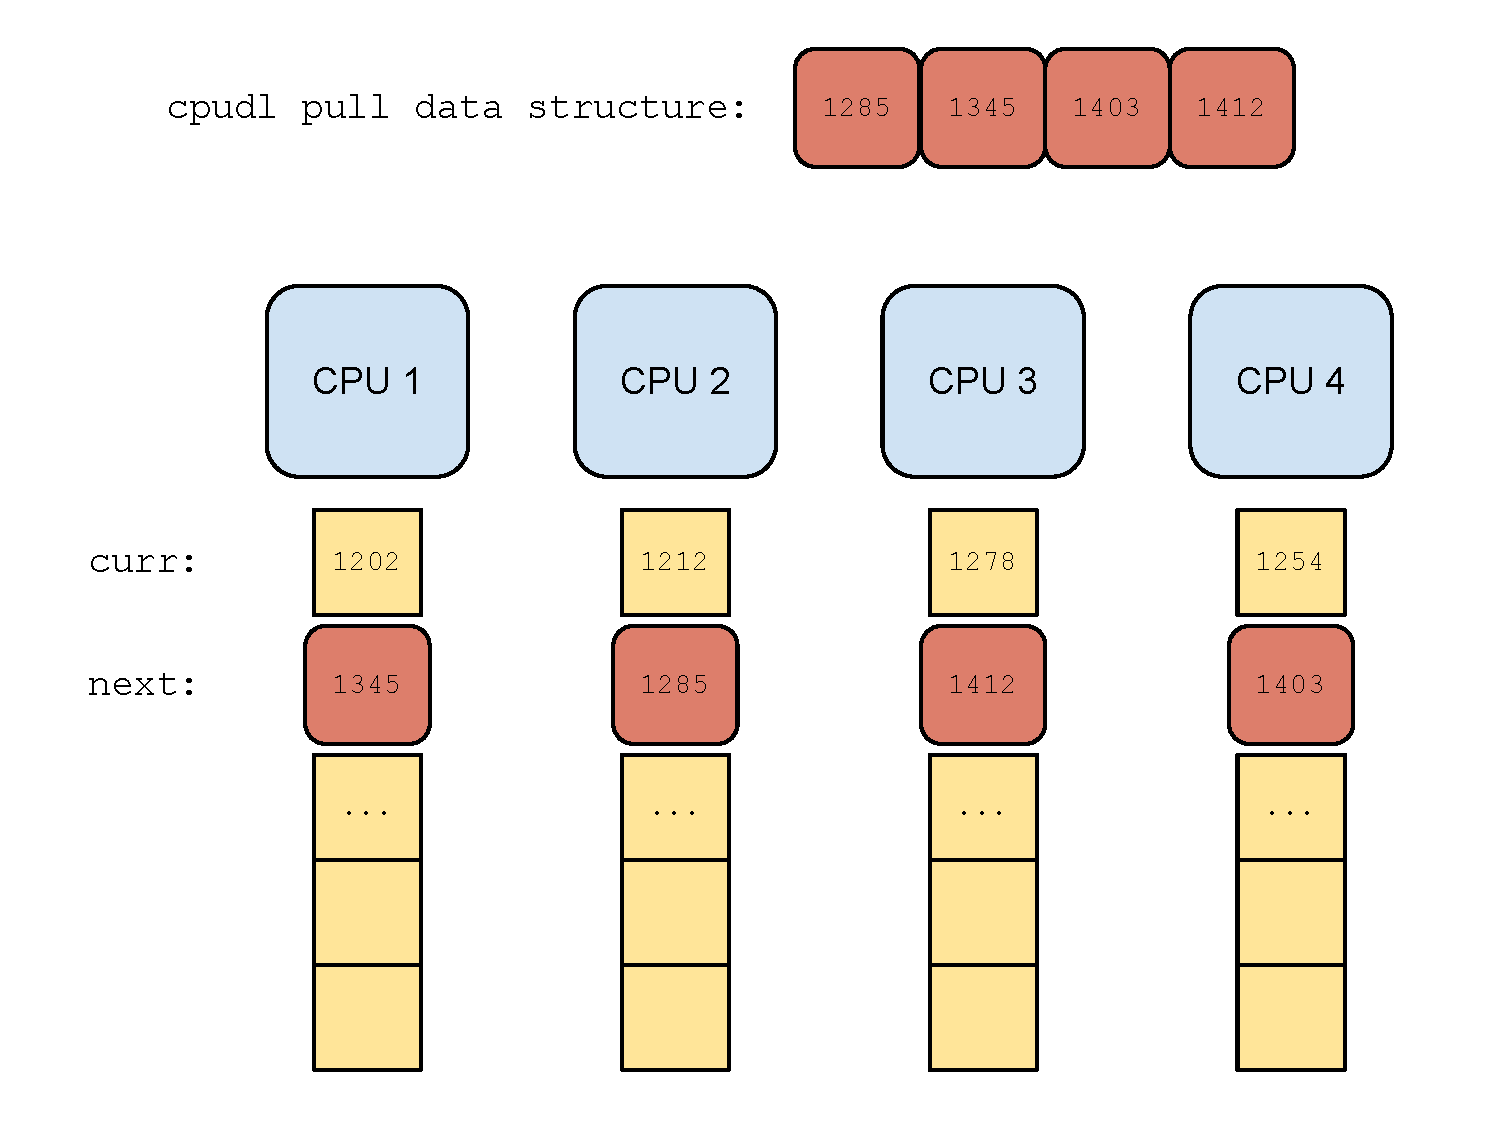
\includegraphics[width=\columnwidth]{images/Pull_cpudl}
    \caption{\texttt{cpudl} structure for \emph{pull} operation.}
    \label{fig:cpudl_pull}
\end{figure}

All the data structures presented in the previous sections have been developed
with a hook to a deadline compare function: this way we can use the same
code for both push and pull operations.

The related source code is reported in Appendix~\ref{sec:improved_pull_code}.
